\chapter{Observational strategies: power spectra and images}

\begin{bf}
  \author{Gianni Bernardi (INAF-IRA \& Rhodes University)}\\
  
Abstract\\

This chapter reviews the basics of radio interferometry (van-Citter-Zernike theorem, uv-coverage, image formation calibration) and how they are linked to the measurements of the 21-cm power spectrum and its tomography 
\end{bf}


%\section{Chapter layout}
%\begin{itemize}
%\item review of basics of interferometry: van-Citter-Zernike theorem, $uv$-coverage, image formation;
%\item from visibilities to power spectra (in particular the delay transform approach - some overlap with Trott's chapter);
%\item interferometric calibration: impact on foreground subtraction, calibration errors redundant calibration;
%\item array design: power spectrum vs imaging, minimmum vs maximum redundancy - some overlap with Trott's chapter?;
%\item impact of calibration errors on power spectra;
%\item ionospheric impact/calibration;
%\item 21-cm image tomography;  
%\end{itemize}

\section{Interferometry overview}

\begin{figure}[]
\begin{center}
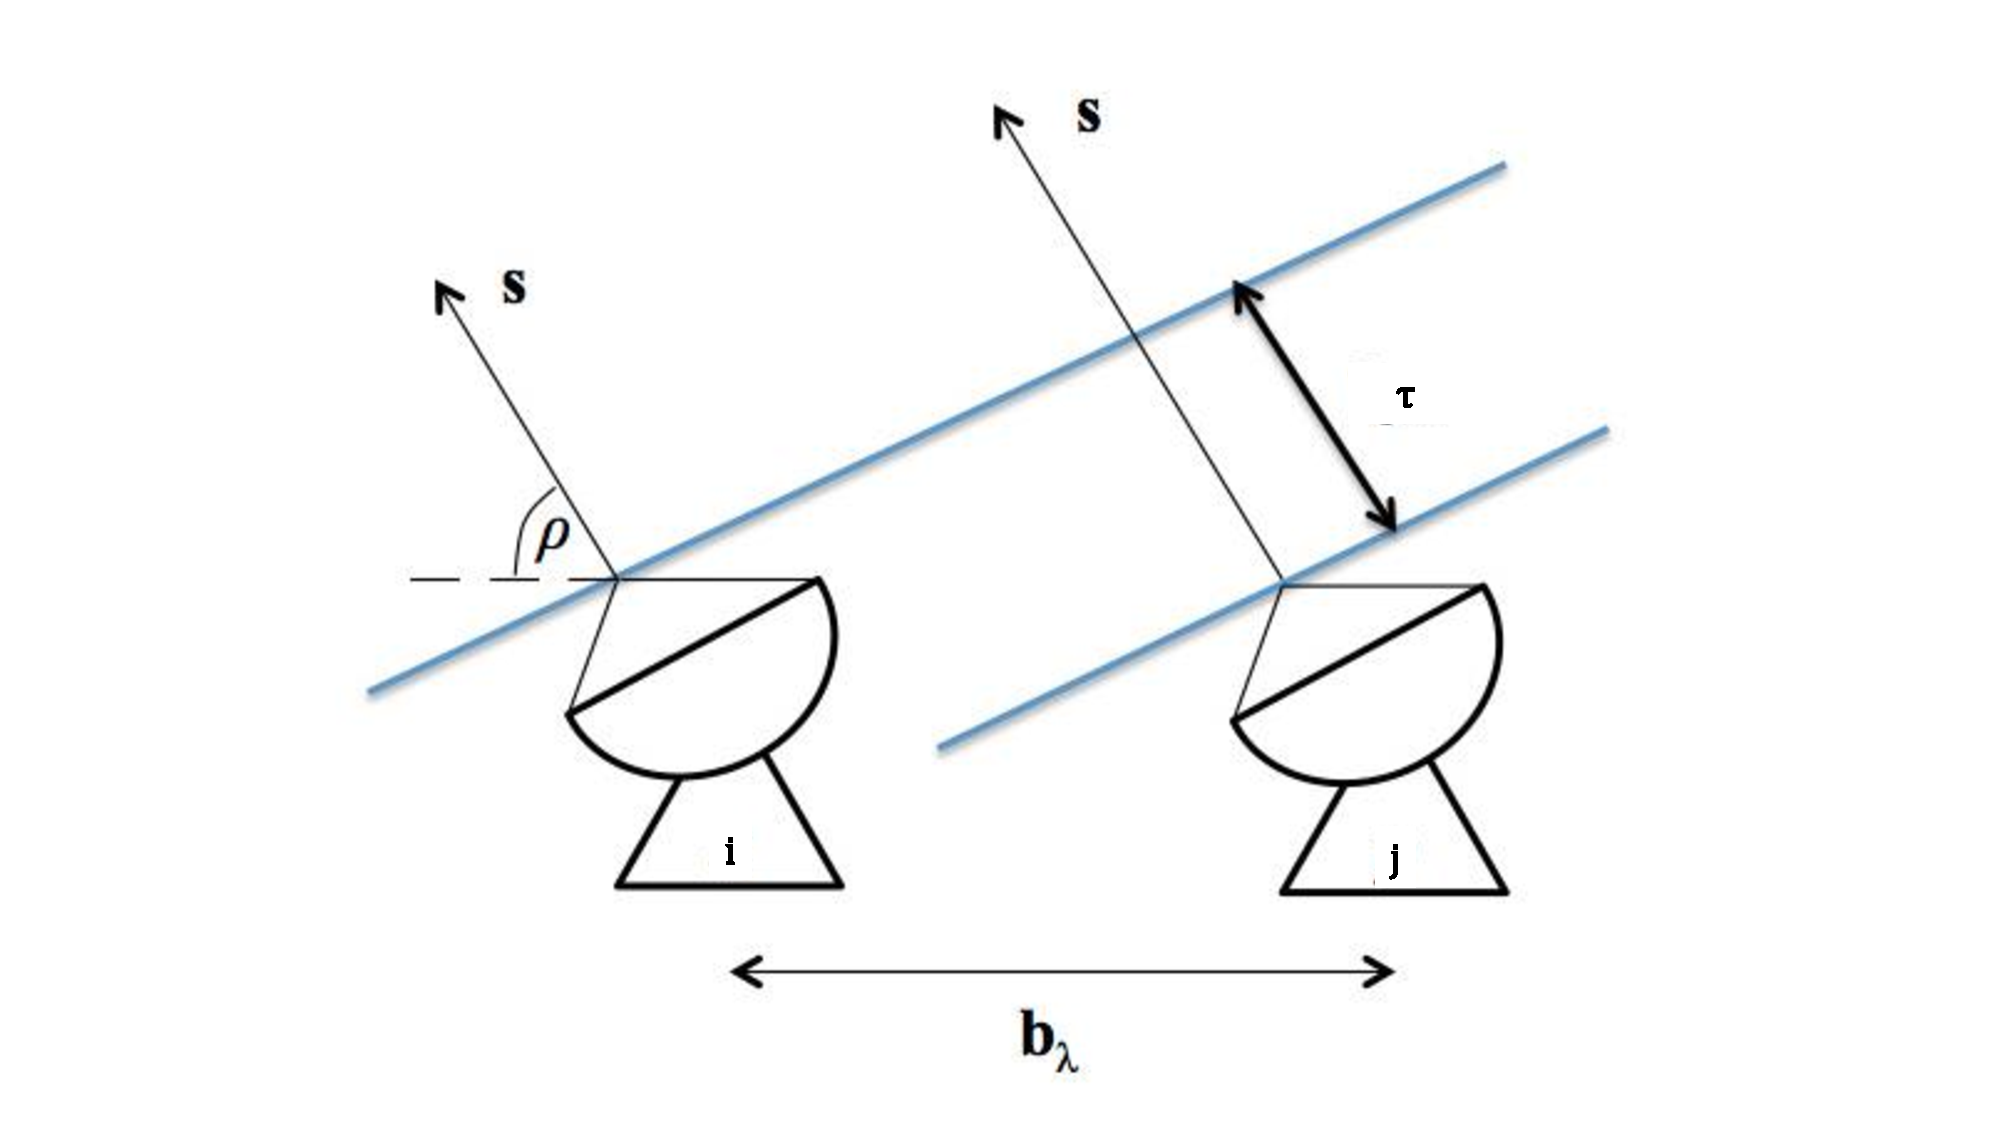
\includegraphics[width=1.\textwidth]{Bernardi/2_element_interferometer}
%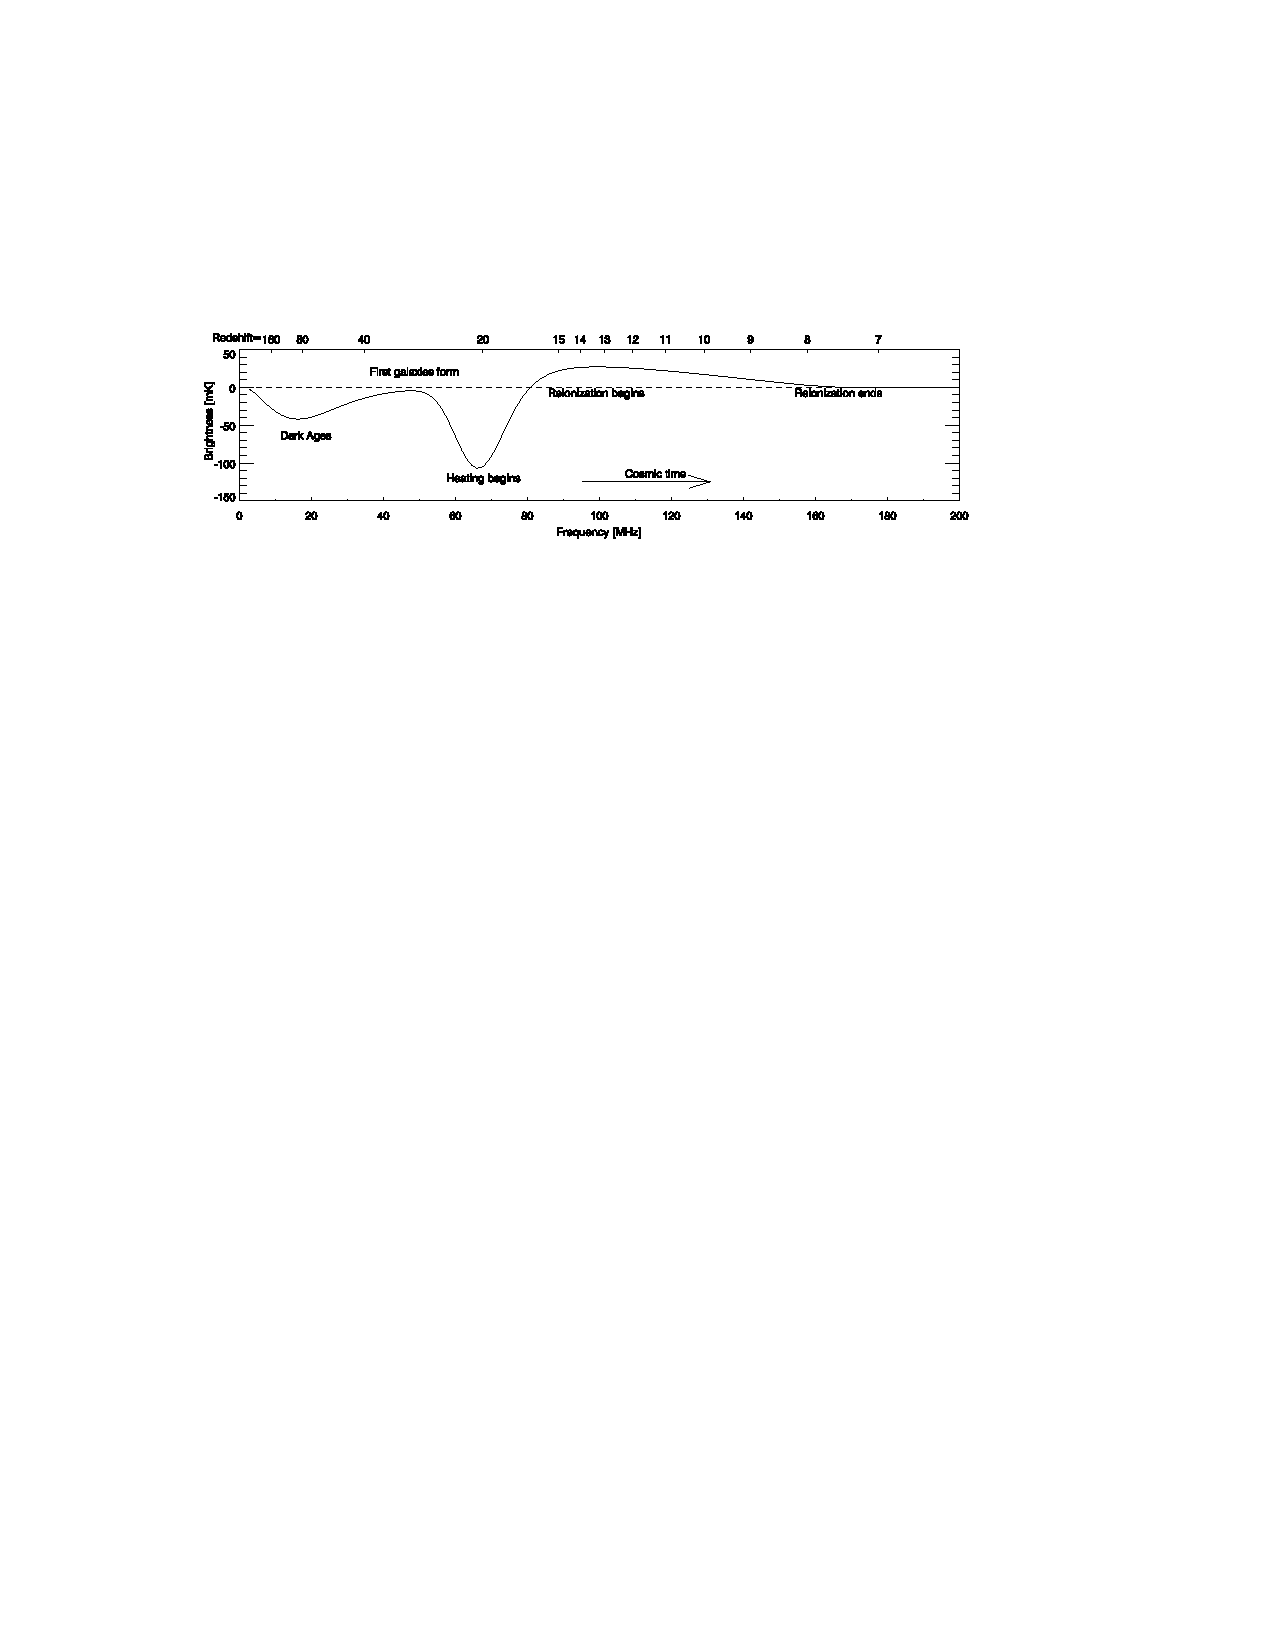
\includegraphics[trim = 0.2cm 0.6cm 0.2cm 0.2cm, scale = 1.0]{Greig/GlobalSignal}
\end{center}
%\caption{A standard schematic of the two element interferometer\footnote{Credit: http://inspirehep.net}.}
\caption{A standard schematic of the two element interferometer.}
\label{fig:fig1}
\end{figure}

The Van Cittert-Zernike theorem expresses the fundamental relationship between the sky spatial brightness (or brightness distribution) $I$ and the quantity measured by an interferometer, i.e. the visibility $V$ (e.g., \cite{TMS}):
\begin{equation}
V_{ij} ({\bf b}, \lambda) = \int_\Omega {\bar I} (\hat{\sigma}, \lambda) \, e^{-2 \pi i {\bf b} \cdot {\hat \sigma}} d {\bf \sigma},
\label{eq:1}
\end{equation}
where ${\bf b}$ is the baseline vector that separates antenna~$i$ and antenna~$j$, and $\hat{sigma}$ is the observing direction (see Figure~\ref{fig:fig1}) and the integral is taken over the source size $\Omega$. The baseline vector is here specified in wavelengths, i.e. ${\bf b} = \frac{{\bf b_{\rm m}}}{\lambda}$, where ${\bf b_{\rm m}}$ is the baseline vector expressed in meters and $\lambda$ is the observing wavelength. It can be seen in Figure~\ref{fig:fig1}, that the celestial signal travels an extra path between the two antennas, and that length corresponds to a geometrical time delay $\tau = {\bf b} \cdot {\hat \sigma}$, where the word ``geometrical" refers to the fact that the delay depends upon the source position in the sky and the relative separation between the two antennas.

The sky brightness distribution does not enter directly in equation~\ref{eq:1}, but filtered by the antenna primary beam response $A$ that depends upon the direction in the sky and the wavelength, i.e. ${\bar I} ({\bf b}, \lambda) = A ({\bf b}, \lambda)  \, I ({\bf b}, \lambda)$. The response of the primary beam attenuates the sky emission away from the pointing direction, effectively reducing the field of view $\theta$ of the instrument. Generally speaking, the size of the field of view is essentially given by the antenna diameter $D$: 
\begin{equation}
\theta \approx \frac{\lambda}{D}.
\label{eq:2}
\end{equation}
Equation~\ref{eq:1} is often re-written in a different coordinate system, i.e. using the components of the baseline vector $(u,v,w)$ and the reciprocal $(l,m,n)$, where $(l,m)$ are the coordinates in the plane on the sky tangent to the observing direction $n$ (for a detailed discussion of coordinate systems see, for example \cite{TMS}). Using this coordinate system, equation~\ref{eq:1} becomes (e.g., \cite{TMS}):
\begin{equation}
V_{ij} (u,v,w, \lambda) = \int_\Omega {\bar I} (l, m, \lambda) \, e^{-2 \pi i (ul + vm + w(n - 1))} \frac {dl \, dm \, dn}{\sqrt{1 - l^2 - m^2}},
\label{eq:3}
\end{equation}
Although low frequency radio observations are intrinsically wide-field, for the purpose of studying the 21~cm observables, we can reduce equation~\ref{eq:3} to a two dimensional Fourier transform:
\begin{equation}
V_{ij} (u,v, \lambda) = \int_\Omega {\bar I} (l, m, \lambda) \, e^{-2 \pi i (ul + vm)} dl \, dm.
\label{eq:4}
\end{equation}
Equation~\ref{eq:4} indicates that an {\it interferometer measures the two dimensional Fourier transform of the spatial sky brightness distribution}. If our goal is to reconstruct the sky brightness distribution, equation~\ref{eq:4} can be inverted into its corresponding Fourier pair:
\begin{equation}
%{\bar I} (l, m, \lambda) = \int_{- \infty}^{+ \infty} V_{ij} (u,v, \lambda) \, e^{2 \pi i (ul + vm)} du \, dv.
{\bar I} (l, m, \lambda) = \int V_{ij} (u,v, \lambda) \, e^{2 \pi i (ul + vm)} du \, dv.
\label{eq:5}
\end{equation}
Equation~\ref{eq:5} is, however, a poor reconstruction of the sky brightness distribution as only one Fourier mode is sampled at a single time instance. Strictly speaking, indeed, all the quantities in equation~\ref{eq:4} and \ref{eq:5} are time variable. In most cases, the time dependence of the primary beam and the sky brightness distribution can be neglected, however, this is not the case for the visibility $V$ as the projection of the baseline vector with respect to the source direction changes significantly throughout a long (e.g. a few hours) track. In this way, many measurements of the visibility coherence function $V$ can be made as $(u,v)$ change with time, allowing for a better reconstruction of the ${\bar I} (l, m, \lambda)$ function. This methods is commonly referred to as {\it filling the $uv$ plane via Earth rotation synthesis} and was invented by \cite{ryle60}. The other (complementary) way to fill the $uv$ plane is to deploy more antennas on the ground in order to increase the number of instantaneous measurements of independent Fourier modes. If $N$ antennas are connected in an interferometric array, $\frac{N (N - 1)}{2}$ instantaneous measurements are made. 

The combination of a large number of antennas and the Earth rotation synthesis, defines the sampling function $S(u,v)$ in the $uv$ plane. In any real case, equation~\ref{eq:5} can therefore be re-written as:
\begin{equation}
{\bar I}_D (l, m, \lambda) = \int S(u,v, \lambda) V (u,v, \lambda) \, e^{2 \pi i (ul + vm)} du \, dv,
\label{eq:6}
\end{equation}
where ${\bar I}_D$ indicates the sky brightness distribution sampled at a finite number of $(u,v)$ points (often termed {\it dirty image}) and where the explicit dependence on the antenna pair was dropped for simplicity. Using the convolution theorem, equation~\ref{eq:6} can be re-written as:
\begin{equation}
{\bar I}_D (l, m, \lambda)  =  \tilde{S \, V} =  {\tilde S} \ast {\tilde V} = {\rm PSF} (l, m, \lambda) \ast {\tilde V} (l, m, \lambda),
\label{eq:7}
\end{equation}
where the tilde indicates the Fourier transform, $\ast$ the convolution operation and PSF is the Point Spread Function, i.e. the response of the interferometric array to a point sources which, in our case, is also the Fourier transform of the $uv$ coverage.

%I will give some examples of sampling functions for different instruments in Section~\ref{sec:design}, however, 
The sampling function always effectively reduces the integral over a finite (often not contiguous) area of the $uv$ plane. In particular, the sampled $uv$ plane is restricted to a minimum $uv$ distance that cannot be shorter than the antenna\footnote{In this chapter I use the words ``antenna" and ``station" interchangeably to indicate the correlated elements even if, in the literature, they are normally used to indicate a dish and and a dipole, or a cluster of dipoles, respectively.} size and the largest separation between antennas, i.e. the maximum baseline ${\bf b}_{\rm max}$. The maximum baseline also sets the maximum angular resolution $\theta_b$:
\begin{equation}
\theta_b \approx \frac{\lambda}{|{\bf b}_{\rm max}|}.
\label{eq:8}
\end{equation}
The incomplete sampling of the $uv$ space leads to a PSF that has ``sidelobes", i.e. nulls and secondary lobes that can often contaminate fainter true sky emission. The best reconstruction of the sky brightness distribution ${\bar I}$ requires deconvolution of the dirty image from the PSF. 




\section{21~cm observables: power spectra and images}
\label{sec:observables}

The ultimate goal of 21~cm observations is to image the spatial distribution of the 21~cm signal as a function of redshift, also known as {\it 21~cm tomography}. Given the curent theoretical predictions, such observations need to achieve mK sensitivity on a few arcminute angular scales (see Chapter 1 in this book). Most of the current arrays, however, only have the sensitivity to perform a statistical detection of the 21~cm signal, i.e. to measure its power spectrum. Given an intensity field $T$, function of the three dimensional spatial coordinate $\bf x$, its power spectrum $P(k)$ is defined as:
\begin{equation}
%\langle {\tilde T}^* ({\bf k}) {\tilde T}({\bf k'}) \rangle = (2 \pi)^3 P({\bf k}) \delta^3({\bf k} - {\bf k}')
\langle {\tilde T}^* ({\bf k}) {\tilde T}({\bf k'}) \rangle = (2 \pi)^3 P(k) \delta^3({\bf k} - {\bf k}')
\label{sec_observables_eq1}
\end{equation}
where $\langle \rangle$ indicates the ensamble average, $\bf k$ is the Fourier conjugate of $\bf x$, tilde the Fourier transform, $^*$ the conjugate operator and $\delta$ the Dirac delta function. In 21~cm observations, power spectra can be computed directly from interferometric image cubes after deconvolution of the dirty image ${\bar I}_D (l,m,\lambda)$ from the point spread function (e.g., \cite{pen09}, \cite{harker10}, \cite{beardsley16}, \cite{patil17}). Alternatively, the 21~cm power spectrum can be estimated directly from the interferometric visibilities. Equation~\ref{eq:4} already shows that the interferometer is a ``natural" spatial power spectrum instrument (e.g., \cite{white99}). Visibilities can be further Fourier transformed along the frequency axis (the so-called {\it delay trasform}, \cite{parsons12a}): 
\begin{equation}
{\tilde V}_{ij} (u,v, \tau) = \int_B {\bar I} (l, m, \nu) \, e^{-2 \pi i \nu \tau} d \nu
\label{sec_observables_eq2}
\end{equation}
where $B$ is the observing bandwidth and $\tau$ is the geometrical delay. The delay transform is therefore proportional to the three dimensional power spectrum (\cite{parsons12b}):
\begin{equation}
P(k) \propto {\tilde V}_{ij} (|{\bf b}|, \tau),
\label{sec_observables_eq3}
\end{equation}
where the proportionality constant transforms the visibility units into power units (\cite{parsons12b}). The observer units $({\bf b},\tau)$ map directly in $k$ modes parallel and perpendicular to the line of sight (e.g., \cite{morales04}):
\begin{equation}
k_\perp = \frac{2 \pi |{\bf b}|}{D_c} = \frac{2 \pi \sqrt{u^2 + v^2}}{D_c}, \,\,\,\,\,\,\,    k_\parallel = \frac{2 \pi f_{21} H_0 E(z)}{c \, (1 + z)^2} \, \tau,
\label{sec_observables_eq4}
\end{equation}
where $D_c$ is the transverse comoving distance, $f_{21} = 1421$~MHz, $H_0$ is the Hubble constant and $E(z) = \sqrt{\Omega)m (1+z)^3 + \Omega_k (1+z)^2 + \Omega_\Lambda}$. Due to the dependence of the geometrical delay upon frequency, equation~\ref{sec_observables_eq3} is only valid for short baselines, typically shorter than a few hundresd meters, for which the geometrical delay is fairly constant across the bandwidth and lines of constant $k_\parallel$ are essentially orthogonal to the $k_\perp$ axis (\cite{parsons12b}).

Equation~\ref{sec_observables_eq2} does not only provide a link between visibilities and three dimensional power spectra, but also introduces the concept of ``horizon limit", i.e. the maximum physical delay allowed $\tau_{\rm max} = \frac{|{\bf b}|}{c}$, where $c$ is the speed of light. The most relevant implication of the existence of an horizon limit is the definition of a region in the two dimensional $(k_\parallel,k_\perp)$ power spectrum space where smooth-spectrum foregrounds are confined, leaving the remaining area  uncontaminated in order to measure the 21~cm signal (the so-called ``Epoch of Reionization (EoR) window", Figure~\ref{fig:fig2}). Foregrounds can therefore be ``avoided" with no requirements for subtraction (e.g., \cite{morales12}, \cite{vedantham12}, \cite{pober13}, \cite{thyagarajan13}; see also Chapter~6 in this book).
\begin{figure}[]
\begin{center}
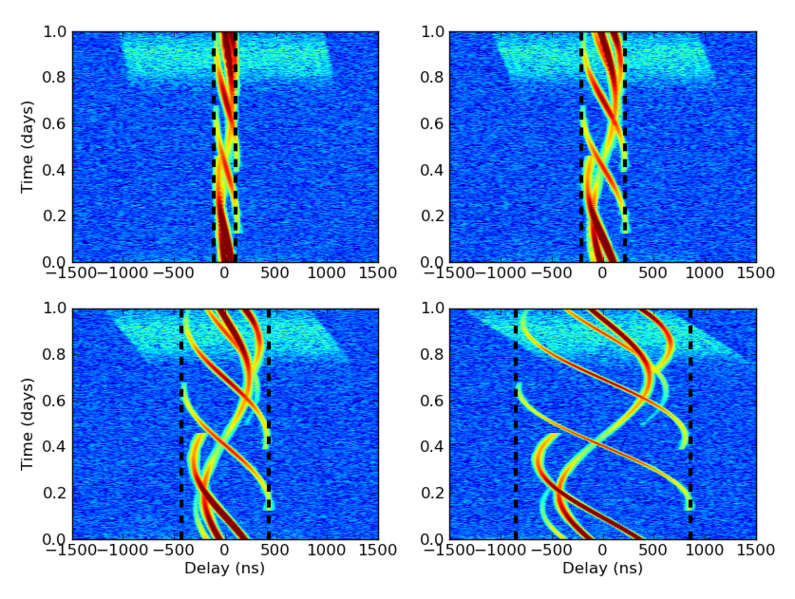
\includegraphics[width=1.\textwidth]{Bernardi/delay_transform}
\end{center}
\caption{Amplitude of delay transformed visibilities as a function of time and delay for a 32 (top let), 64 (top right), 128 (bottom left) and 256~m (bottom right) respectively (from \cite{parsons12a}). A number of smooth spectrum point sources are simulated as foregrounds and their tracks are clearly bound within the horizon limit (black dashed line). The cyan emission is a fiducial 21~cm model that has power at high delays regardless of the baseline length.}
\label{fig:fig2}
\end{figure}
The choice of a foreground avoidance strategy versus subtraction plays an important role in planning an experiment, its related observing strategy and the array calibration strategy.

The requirements for image tomography are the same as for high brightness sensitivity observations of diffuse emission like the Cosmic Microwave Background (e.g. \cite{VSA}, \cite{DASI}, \cite{CBI}). The 21~cm spatial distribution throughout cosmic reionization has structures on 5-10 arcminutes up to degree scales (e.g., \cite{mellema}, \cite{zaroubi}). In order to image 21~cm fluctuations, a maximum baseline of the order of a few km gives a resolution of a few arcminutes in the $100-200$~MHz range, together with filled $uv$ plane in order to accurately reconstruct their complex spatial structure. A filled $uv$ plane also leads to a PSF with very low sidelobes, making the deconvolution process easier. The most stringent requirements for image tomography remain the accurate foregrond separation and, as I will review in the next section, the related instrumental calibration.



%\section{Challenges in 21~cm observations: interferometric calibration in presence of bright foreground emission, wide fields of view, ionosphere}
\section{Interferometric calibration and 21~cm observations}
\label{sec:challenges}

Celestial signals always experience a corruption due to the non-ideal instrumental response that needs to be corrected for a posteriori, in a process that is known as interferometric calibration. Calibration relies on the definition of a data model where the corruptions are described by antenna based quantities known as Jones matrices. The data model is known as the interferometric measurement equation (\cite{hamaker96},\cite{smirnov11}) that will be summarized in the following.

If antenna $1$ and antenna $2$ measure two orthogonal, linear polarizations $x$ and $y$, the cross-polarization visibility products can be grouped in a $2 \times 2$ matrix ${\bf V}$
\begin{equation}
    {\bf V}_{12} (u,v,\lambda) \equiv 
    \left[ 
    \begin{array}{cc}
    V_{12,xx} (u,v,\lambda) & V_{12,xy} (u,v,\lambda) \\
    V_{12,yx} (u,v,\lambda) & V_{12,yy} (u,v,\lambda) \\
    \end{array}
    \right].   
\label{eq:sec:1}
\end{equation} 
The sky brightness distribution $I$ can also be written as a $2 \times 2$ matrix ${\bf B}$ using the Stokes parameters as a polarization basis:
\begin{equation}
    {\bf B}_I (l,m,\lambda) \equiv 
    \left[
    \begin{array}{cc}
    I (l,m,\lambda) + Q (l,m,\lambda) & U (l,m,\lambda) + iV (l,m,\lambda) \\
    U (l,m,\lambda) - iV (l,m,\lambda) & I (l,m,\lambda) - Q (l,m,\lambda) \\
    \end{array}
    \right].   
\label{eq:sec:2}
\end{equation} 
At this point, equation~\ref{eq:3} can be written by including the corruptions represented by the Jones matrices $J$ (\cite{hamaker96},\cite{smirnov11}):
\begin{equation}
{\bf V}_{12} (u,v,\lambda) = {\bf J}_1 \left( \int_\Omega {\bf B}_I (l, m, \lambda) \, e^{-2 \pi i (ul + vm)} dl \, dm  \right) {\bf J}_2^H
\label{eq:sec:3}
\end{equation} 
Equation~\ref{eq:sec:3} is known as the measurement equation and is the core of interferometric calibration. For an array with $N$ antennas, equation~\ref{eq:sec:3} can be written for each of the $\frac{N (N - 1)}{2}$ visibilities forming an overdetermined system of equations. The development of calibration algorithms is a very active research line (\cite{mitchell08}, \cite{kazemi11}, \cite{tasse14}, \cite{yatawatta15}, \cite{smirnov15}) although beyond the scope of this chapter and we mention it here for completeness.
The solution of the system of calibration equations requires some knowledge of the sky brightness distribution ${\bf B}_I$, or a {\it sky model}. Traditionally this is achieved by observing a calibration source, i.e. a bright, unresolved point source with known spectral and polarization properties. Calibration solutions are then applied to the observed field that, in turn, is then used to improve the sky model ${\bf B}_I$ which, in turn, leads to more accurate calibration solutions $J$ in the loop that is traditionally called {\it self calibration} (\cite{cornwell81}, \cite{pearson84}). This approach can lead to a highly accurate calibration (e.g., \cite{bernardi10}, \cite{smirnov11b}).

The advantage of the measurement equation is that it can factorize different physical terms into different matrices. For example, the frequency response of the electronic filters and its time variations essentially affects only the two polarization response and are modeled with a diagonal Jones matrix $B$:
\begin{equation}
    {\bf B} (t,\lambda) \equiv 
    \left[
    \begin{array}{cc}
    b_x (t,\lambda) 	& 	0 	\\
    0 		& b_y (t,\lambda) 	\\
    \end{array}
    \right],   
\label{eq:sec:4}
\end{equation} 
whereas the undesired instrumental leakage between the two orthogonal polarized is represented by a $D$ Jones matrix of the form:
\begin{equation}
    {\bf D} (t,\lambda) \equiv 
    \left[
    \begin{array}{cc}
    1	 		& d_x (t,\lambda)	\\
    -d_y (t,\nu)	& 1 	\\
    \end{array}
    \right],   
\label{eq:sec:5}
\end{equation} 
and the measurement equation can be written as:
\begin{equation}
{\bf V}_{12} (u,v,\lambda) = {\bf B}_1 \, {\bf D}_1 \left( \int_\Omega {\bf B}_I (l, m, \lambda) \, e^{-2 \pi i (ul + vm)} dl \, dm  \right) {\bf D}_2^H  \, {\bf B}_2^H.
\label{eq:sec:6}
\end{equation}
We note that, in principle, the primary beam response should appear as an additional $2 \times 2$ Jones matrix before the $D$ matrix. For our pedagogical purposes, we assume that it can be incorporated in the $B$ matrix, although we later illustrate an exception to this assumption.

Retaining only the first order terms, equation~\ref{eq:sec:6} can be written as (\cite{sault96}):
\begin{eqnarray}
V_{12,xx} (u,v,\lambda) & = & b_{1,x} \, b_{2,x}^* [V_I (u,v,\lambda) - V_Q (u,v,\lambda)]\\
V_{12,xy} (u,v,\lambda) & = & b_{1,x} \, b_{2,y}^* [(d_{1,x} - d_{2,y}^*) V_I (u,v,\lambda) + V_U (u,v,\lambda) + iV_V (u,v,\lambda)]	\\
V_{12,yx} (u,v,\lambda) & = & b_{1,y} \, b_{2,x}^* [(d_{2,x} - d_{1,y}^*) V_I (u,v,\lambda) + V_U (u,v,\lambda) - iV_V (u,v,\lambda)]	\\
V_{12,yy} (u,v,\lambda) & = & b_{1,y} \, b_{2,y}^* [V_I (u,v,\lambda) - V_Q (u,v,\lambda)],
\label{eq:sec:7}
\end{eqnarray}
where we dropped the explicit dependence on time and wavelength from the Jones matrices for notation clarity and where $V_{i=I, Q, U, V}$ are the Fourier transforms of the sky brightness matrix $B$.

This form of the measurement equation offers an intuitive understanding as to why calibration is so important in 21~cm observations. The observed visibilities are essentially a measurement of foreground emission and, in the ideal case, their amplitudes would vary smoothly with frequency, enabling  either their avoidance or subtraction. However, the instrumental response inevitably corrupts this smoothness in several ways: because the telescope primary beam is not sufficiently smooth in frequency, because of the filter response or because of reflection along the signal path. Calibration attempts to restore the intrinsic foreground frequency smoothness, however, calibration errors (i.e., deviations from the true $B$ solutions) will corrupt the foreground frequency smoothness. In practice, calibration errors result into foreground power leaking out of the horizon limit and jeopardizing (part of) the EoR window. The corruption of the foreground frequency smoothness will limit the accuracy of any subtraction method (see {\bf Chapter~!!!}). {\it The effectiveness of foreground separation, proven in ideal cases, depends significantly on the accuracy of interferometric calibration.}

There are a few topics of active research in improving the accuracy of interferometric calibration:
%
\begin{itemize}
\item {\it sky models}. Ideally, the sky brightness model matrix ${\bf B}_I$ (equation~\ref{eq:sec:6} and \ref{eq:sec:7}) should include the whole sky emission. This is pratically impossible as part of the sky signal is the unknown that we want to discover (the 21~cm signal) and part of the signal has not been observed before or, even if observed, its detailed properties are not know sufficiently well. 
\begin{figure}[]
\begin{center}
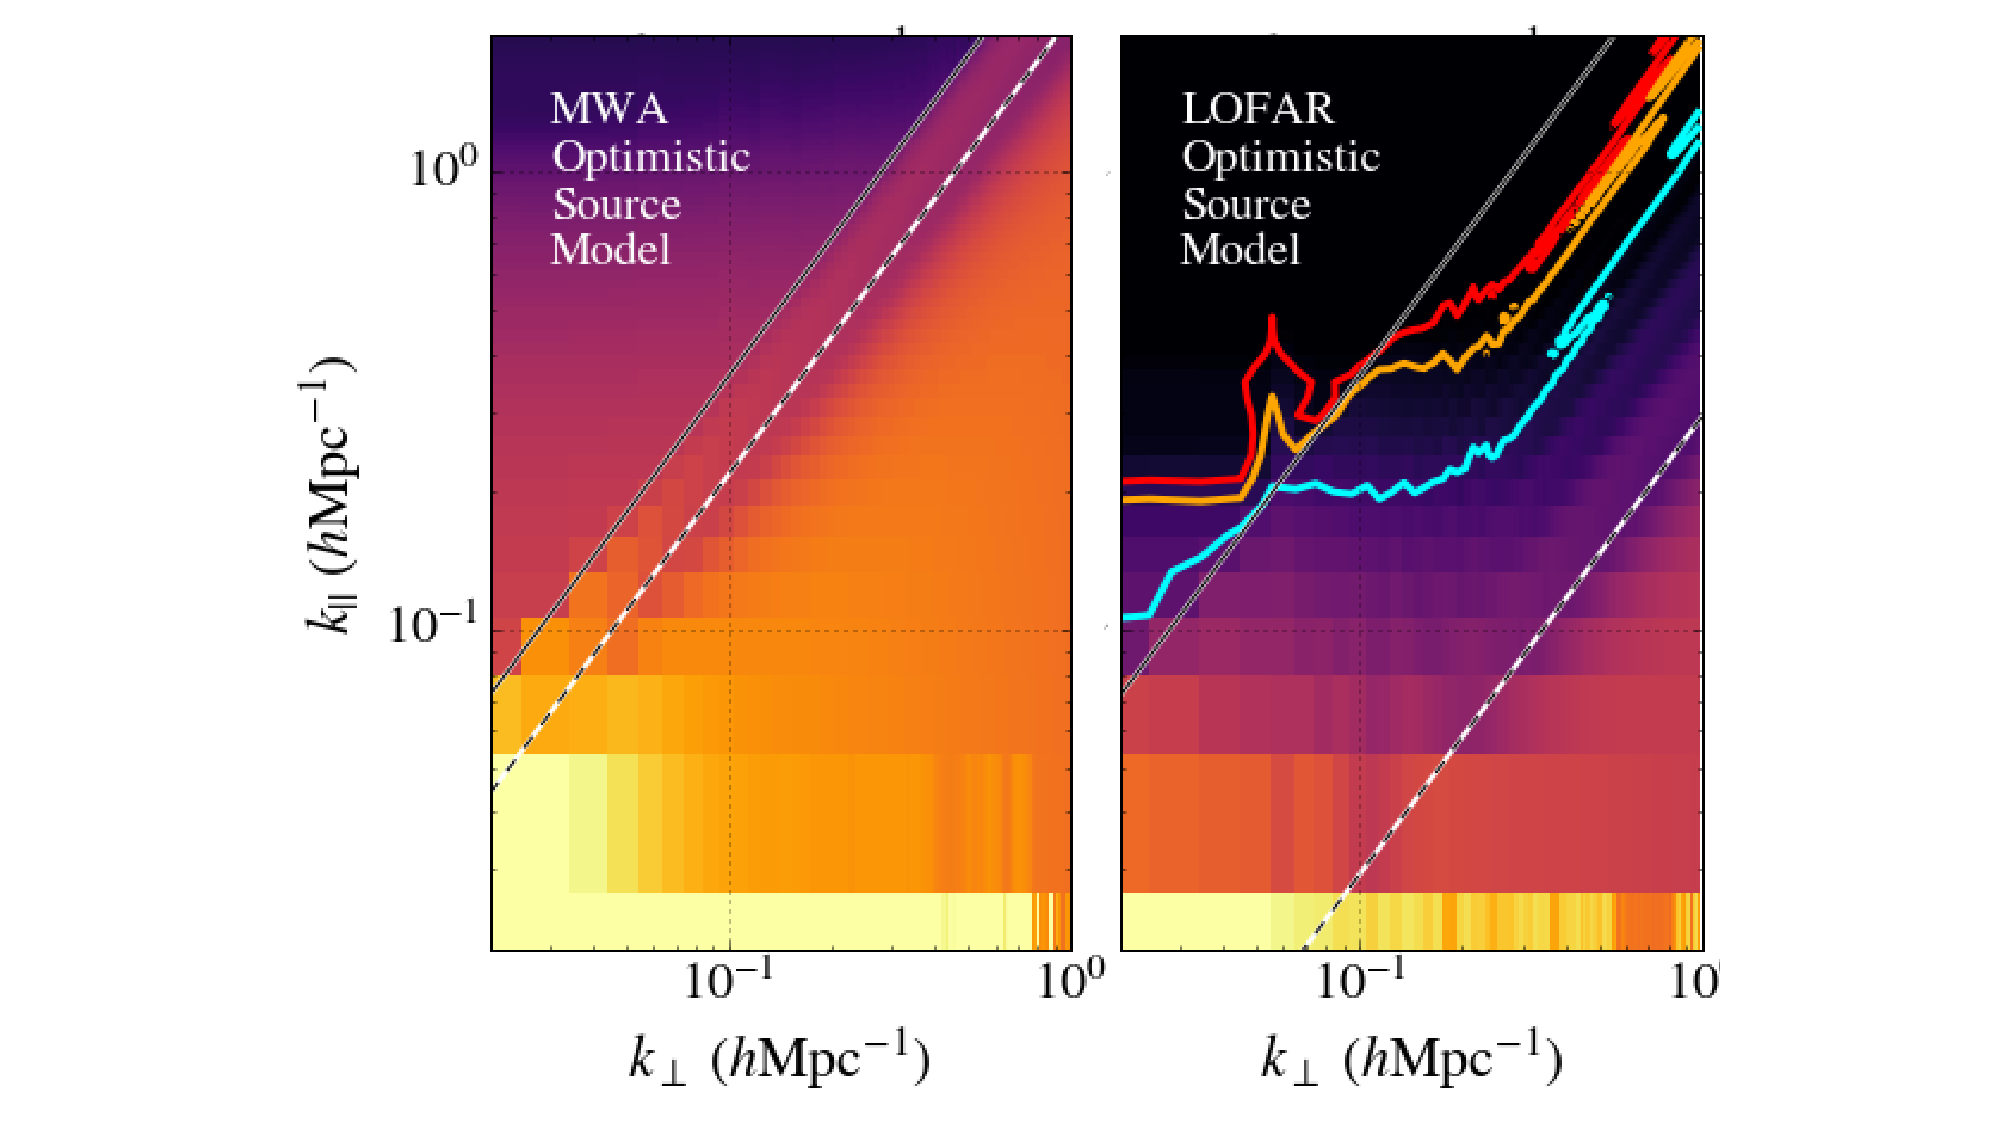
\includegraphics[width=1.\textwidth]{Bernardi/calibration_errors}
\end{center}
\caption{Example of power spectrum bias introduced by calibration errors due to incomplete sky models for the Murchison Widefield Array (MWA, left) and the Low Frequency Aray (LOFAR, right) cases respectively (from \cite{ewall-wice17}). Power spectra are shown in their two dimensional $(k_\perp,k_\parallel)$ form in order to show the foreground dominated region below the horizon limit (grey solid line). Cyan, orange and red lines are the lines where a fiducial 21~cm model is one, five and ten times higher than the power spectrum bias level. In an ideal case with perfectly smooth foregrounds and no calibration errors, the 21~cm power sepctrum should be detectable just outside the horizon limit. The errors introduced by an incomplete sky model lead to a foreground power leakage in the EoR window which, in the MWA case, may completely prevent a detection.}
\label{fig:fig_added}
\end{figure}

Efforts to achieve the most accurate calibration include in the brightness matrix $B_I$ thousands of compact sources in an aread larger than the telescope field of view (e.g., \cite{yatawatta13}. This sky model may still be insufficient as it does not include sources over the whole sky nor Galactic diffuse emission. Galactic emission contributes to most of the power on  angular scales $\theta > 10-20$~arcmin (\cite{bernardi09}, \cite{choudhuri17}), therefore a compact sources sky model is not adequate for baselines shorter than a few tens of meters. Excluding short baselines from the calibration solutions would prevent the problem but can bias the solution (\cite{patil16}) if the system of calibration equation is not properly regularized (\cite{sardabaradi19}).

Another form of sky model incompleteness is related to angular resolution: due its finite resolution, sources that are not completely unresolved are nevertheless treated as point-like and this too biases the calibration solutions, leading to an excess of foreground contamination in the EoR window (\cite{procopio17}). 

\cite{grobler14}, \cite{wijnholds16} and \cite{grobler16} show that effect of sky model incompleteness on calibration eventually leads to artifacts in the form of ghost-like sources in interferometric images, most of the times fainter than the image noise level. They also show that the ghost pattern is stronger for regularly spaced arrays and if the sky model is more incomplete. \cite{ewall-wice17} and \cite{barry16} formalize the effect of incomplete sky models on calibration as a leakage of foreground power in the EoR window.

Significant effort is currently ongoing in order to improve the all-sky compact-source model via wider and deeper low frequency surveys (e.g., \cite{hurley-walker17}, \cite{intema17}, \cite{shimwell19}), more accurate low frequency catalogues (\cite{carroll16}) and even improvements of the Galactic diffuse emission observations (\cite{zheng17}, \cite{dowell17}). Some of the calibration strategies described in the next sections may, however, mitigate the requirements of extremely accurate sky models;

\item {\it instrument/primary beam models}. A complete knowledge of a sky model may not be, by itself, sufficient for an accurate calibration of 21~cm observations as the brightness matrix $B_I$ appears in the calibration equation multiplied by the antenna primary beam (equation~\ref{eq:sec:3} and \ref{eq:4}) and the measurement of an intrinsic sky model requires the separation from the primary beam effect. 

Unlike steerable dishes, most 21~cm interferometers are constituted of dipoles fixed on the ground, in some cases clustered together to form tiles or stations that can digitally pointed in a sky direction via a physical delay (e.g., like the MWA and LOFAR arrays, see Section~\ref{sec:design}). As station beams are formed to track the source on the sky, the station projected area changes with time and the shape of the primay beam changes significantly (Figure~\ref{fig:fig3}). This effect leads to time variable sky models with variations that are larger away from the pointing direction due to the large variations in the sidelobe pattern. For examples, sky sources that are well within the main lobe of the primary beam in Figure~\ref{fig:fig3} will experience relatively negligible variations throughout an observation, the opposite will occur to sources located well outside the main lobe as the enter and exit different sidelobes.

Primary beams are also frequency variable and, at first order, their size scales with wavelength (similar to the angular resolution, equation~\ref{eq:2}), i.e. rather smoothly. However, in the sidelobe region, such variation becomes rather abrupt as the sidelobe pattern changes too, therefore the source can be at the peak of a sidelobe at a certain frequency and in the sidelobe null at another frequency. As a final remark, stations are not perfectly equal to each other, due to manifacturing reasons or mutual coupling between their elements (e.g., \cite{sokolowski17}), therefore the sky brightness matrix $B_I$ is potentially different for each baseline as the primary beams are different. The left panel of Figure~\ref{fig:fig3} attempt to quantify this effect in a simulated case: variations in the sidelobe region can be as large as $\sim 30\%$.

If not accurately modeled and taken into account, the aforementioned effects can bias the calibration solution and, again, corrupt the foreground smoothness.  \cite{bhatnagar08}, \cite{sullivan12} and \cite{tasse13} and have developed methods to incorporate time and frequency variable primary beams in interferometric images, however, the accuracy of the correction is limited by the accurace of the primary beam model. Increasing effort is therefore being placed in accurante modeling and measuring primary beams (e.g., \cite{pupillo15}, \cite{deleraacedo17}, \cite{jacobs17}, \cite{deleraacedo18});
\begin{figure}[]
\begin{center}
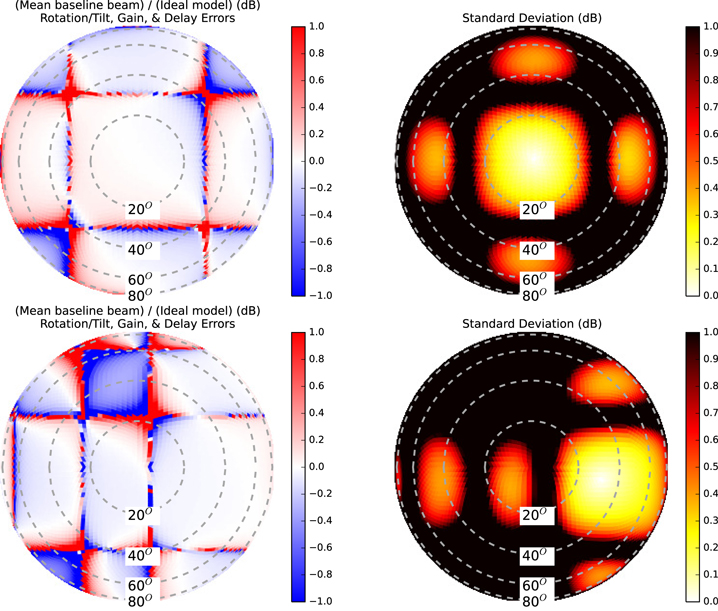
\includegraphics[width=1.\textwidth]{Bernardi/mwa_beams_err}
\end{center}
\caption{Example of primary beam variations as the MWA station points at zenith (top right) and $\sim 30^\circ$ away from zenith (bottom right) at 150~MHz. The left column shows the fractional variation of individual station beam models, with respect to the nominal primary beam (right column, from \cite{neben16}. It is visibile how different sidelob pattern is when pointing towards two different directions. It should also be noticed that the magnitude of the first lobe is at the $\sim 10\%$ level and the large null areas around the lobes. The specific pattern is due to the regular shape of the MWA station, where 16 dipoles are arrange in a square $4 \times 4$ grid.}
\label{fig:fig3}
\end{figure}


\item {\it polarization leakage calibration}. Equation~\ref{eq:sec:3} and \ref{eq:sec:7} show that, even if the 21~cm signal is unpolarized, care needs to be taken against the contamination from polarized foreground emission. Most point sources are unpolarized below 200~MHz (\cite{bernardi13}, \cite{lenc16}, \cite{vaneck18}), therefore the assumption of an unpolarized sky model is well justified. However, errors in the matrix $B$ different between the $xx$ and $yy$ polarizations would lead to polarized emission to leak into total intensity, particularly on short baselines, where polarized foreground emission is brighter (\cite{bernardi09}, \cite{iacobelli13}, \cite{jelic15}, \cite{lenc16}). Polarized foregrounds Faraday rotated by the intersetllar medium that leak to total intensity may be a severe contamination of the 21~cm signal (e.g., \cite{jelic10}, \cite{moore13}, \cite{nunhokee17}).

Even if calibration errors are negligible, low frequency antennas have a non negligible polarized response across their wide field of view. If we call the Jones matrix that represents the polarized primary beam response $E \equiv E (l,m,\lambda)$, its associate measurement equation can be written as (\cite{nunhokee17}):
\begin{eqnarray}
    \left[ 
    \begin{array}{cc}
    V_{12,I} (u,v,\lambda)\\
    V_{12,Q} (u,v,\lambda)\\
    V_{12,U} (u,v,\lambda)\\
    V_{12,V} (u,v,\lambda)
    \end{array}
    \right] & = & \int_\Omega{ {\bf S}^{-1} [ {\bf E}_1 \otimes {\bf E}_2^H ] {\bf S} 
    \left[ 
    \begin{array}{cc}
    I (l,m,\lambda)\\
    Q (l,m,\lambda)\\
    U (l,m,\lambda)\\
    V (l,m,\lambda)
    \end{array}
    \right]
     \, e^{-2 \pi i (ul + vm)} dl \, dm } = \nonumber \\
     & = & \int_\Omega{ {\bf A} (l,m,\lambda) 
    \left[ 
    \begin{array}{cc}
    I (l,m,\lambda)\\
    Q (l,m,\lambda)\\
    U (l,m,\lambda)\\
    V (l,m,\lambda)
    \end{array}
    \right]
     \, e^{-2 \pi i (ul + vm)} dl \, dm },
\label{eq:sec:8}
\end{eqnarray} 
where ${\bf S}$ is the matrix that relates the intrisic Stokes parameters to the observer $-y$ frame, $\otimes$ is the outer product. The visibilities are written as a four-element vector as this form shows that the outer product of the beam Jones matrices maps the intrinsic Stoke parameters into the observed ones: 
\begin{eqnarray}
    \left(
    \begin{array}{cccc}
    I' \leftarrow I & I' \leftarrow Q & I' \leftarrow U & I' \leftarrow V \\
    Q' \leftarrow I & Q' \leftarrow Q & Q' \leftarrow U & Q' \leftarrow V \\
    U' \leftarrow I & U' \leftarrow Q & U' \leftarrow U & U' \leftarrow V \\
    V' \leftarrow I & V' \leftarrow Q & V' \leftarrow U & V' \leftarrow V \\
    \end{array}
    \right).
\label{eq:sec:8}
\end{eqnarray} 
The first raw of the matrix shows how the four intrisinc Stokes parameters contribute to the observed total intensity and, therefore, how polarized foregrounds leak into the 21~cm signal even in absence of any calibration errors: any polarized signal (Stokes $Q$ and $U$) will contaminate the observed total intensity signal, and the magnitude of the contamination increases away from the ponting direction. An example of $\bf A$ matrix is shonw in Figure~\ref{fig:fig4}.

Calibration of the polarization leakage remains a challenging task. It can be mitigated by extending the sky model to include polarization (e.g. \cite{geil11}), although modeling the diffuse Galactic foreground - the brightest component - is not straightforward and requires accurate imaging. \cite{nunhokee17} showed that also polarized foregrounds may be avoided if they are not highly Faraday rotated by the interestellar medium, although a more extensive characterization of polarized foreground properties is needed.
\begin{figure}[]
\begin{center}
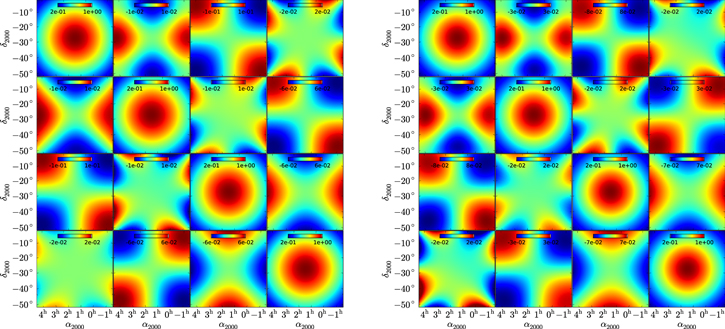
\includegraphics[width=1.\textwidth]{Bernardi/polarized_beam_leakage}
\end{center}
\caption{Examples of ${\bf A}$ matrices at 130 (left) and 150~MHz respectively (from \cite{nunhokee17}). The matrix maps the intrinsic Stokes parameters into observed ones: the diagonal terms represent the expected primary beam shapes, whereas the off-diagonal terms represents leakage terms. The second, the third and the fourth element of the first row show how Stokes parameters $Q$, $U$ and $V$ respectively contaminate the total intensity signal.}
\label{fig:fig4}
\end{figure}



\item {\it ionospheric distortions}
\end{itemize}






\subsection{Direction dependent calibration}

In the previous section I have summarized the calibration equations and the main effects that lead to calibration errors that, in turn, may jeopardize foreground separation. The calibration formalism describe 

\subsection{Redundant calibration}

An interferometric array where most of the baselines have the same length and orientation is called {\it redundant} as they measure the same Fourier mode of the sky brightness distribution. Redundant array configurations are often not appealing as they have poor imaging performances as they do not measure sufficient Fourier modes to reconstruct accurate sky images. However, a maximally redundant array where the antennas are laid out in a regularly spaced square grid offers the maximum power spectrum sensitivity on the $k_\perp$ modes corresponding to the most numerous baselines. This criterium has inspired the highly redundant layouts of the MIT Epoch of Reionization experiment (\cite{zheng14}), the Precision Array to Probe the Epoch of Reionization (PAPER, \cite{parsons12b}) and partly driven the updated MWA.

One of the advantages of a redundant array is that it enables a different calibration strategy called {\it redundant calibration}. In redundant calibration the form of the measurement equation does not change and can be written, for a single polarization, like equation~\ref{eq:sec:7}:
\begin{equation}
V_{12,xx} (u,v,\lambda) = b_{1,x} \, b_{2,x}^* y_{12,xx} (u,v,\lambda),
\label{eq:sec:9}
\end{equation}
with the difference now that the model visibility $y$ is not tied to a sky model, but it is solved for, simply assuming that it is the same for each group of redundant baselines {\cite{wieringa92}, \cite{liu10}). In other words, redundant calibration is independent on the sky model and, therefore, bypasses entirely the biases related to sky model incompleteness described in Section~\ref{sec:challenges}. However, as redundant calibration is not tied to any physical (i.e. sky-based) spatial or spectral model, its solutions have degeneracies that need to be solved for by using a sky model (e.g., \cite{zheng14}, \cite{byrne19}). In particular, spectral calibration, which is critical for foreground separation, cannot currently be obtained using redundant calibration and requires a sky-based calibration. \cite{byrne19} suggest that sky model incompleteness can bias this calibration step, in a way similar to what happens with a traditional calibration scheme.

Redundant calibration is also prone to effects that break the assumption of redundancy, the most common being errors in the antenna positions and different primary beams for different antennas. Even if antenna position errors can be reduced to have a negligible impact on redundant calibration \cite{joseph18}, the effect of primary beam variations amongts the different antennas on redundant calibration is still largely unknown. {\bf Comment on the limitations of redundant calibration to treat polarization.}


\section{Array design and observing strategies}
\label{sec:design}

\begin{figure}[]
\begin{center}
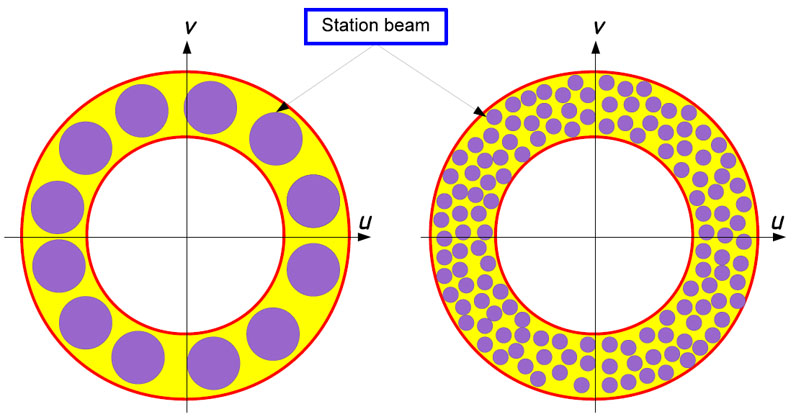
\includegraphics[width=1.\textwidth]{Bernardi/uv_footprint}
\end{center}
\caption{Cartoon illustration of the $uv$ footprint due to the primary beam.}
\label{fig:fig4}
\end{figure}
I will conclude this chapter by discussing how the various interferometric effects discussed so far impact the choice of array designs and the consequent observing strategies. \cite{morales05} and \cite{parsons12b}, for example, investigate how instrumental choices like the array layout, the antenna size and the bandwidth (do not) affect the 21~cm power spectrum spectrum. Here I would rather like to emphasize the interdependence between instrumental choices and calibration and foreground separation strategies. If the total collecting area is kept fixed, there are two main elements that impact calibration and foreground separation:
\begin{itemize}
\item {\it station size}. The choice of station size determines the minimum $k_\perp$ value accessible and the footprint of each $uv$ measurement. Indeed each visibility is not a single point in the $uv$ plane but has a footprint corresponding to the two dimensional Fourier transform of the primary beam. This can be seen using the convolution theorem to re-write equation~\ref{eq:1}: 
\begin{equation}
V_{ij} ({\bf b}, \lambda) = \tilde{A} ({\bf b}, \lambda) \ast \tilde{I} ({\bf b}, \lambda).
\end{equation}

\item {\it array layout} Beyond the obvious sensitivity requirement, decisions need to be taken as to which layout to adopt, which antenna size and these choice are intrinsically related to calibration and foreground separation strategies. For instance a filled $uv$-coverage (between the minimum and the maximum station separation) is highly desirable for imaging, modeling and subtracting foregrounds. It is not a stringent requirement for power spectrum measurement and in the avoidance strategy. 
\end{itemize}



As examples, I will use four existing low frequency arrays that, concidentally, span the range of parameters of interest:

\begin{itemize}
\item effect of the field of view, calibratability, uv cell, drift scan versus tracking, suppression of sources outside the main lobe ionosphere
\item uv coverage choices power spectra vs images, redundant vs pseud random (reconstructing sky brightness), minimum/maximum k mode accessible... avoidance (compact) vs subtraction (less compact)
\item obviously sensitivity

\item {\it Low Frequency Array (LOFAR)}. LOFAR is an array mainly located in The Nerthelands but it include also remote stations acroos Europe. Each station

\item Murchison Widefield Array (MWA)

\item Precision Array to Probe the Epoch of Reionization (PAPER)

\item Hydrogen Epoch of Reionization Array (HERA)

\item Square Kilomtre Array (SKA)

\end{itemize}


%Lorem ipsum dolor sit amet, consectetur adipiscing elit. Duis eu egestas erat. Maecenas tincidunt lacinia tincidunt. Mauris id lectus nec neque feugiat condimentum vitae at diam. In vel orci nunc, non commodo mauris. Vivamus ipsum enim, vulputate quis pharetra non, molestie quis felis. Vivamus porttitor placerat turpis at accumsan. Nunc tortor velit, faucibus a rhoncus nec, blandit non elit. Nam consectetur lectus eu nisi blandit dapibus rhoncus dui tempus. Mauris fermentum dolor vel ipsum vulputate sit amet ultricies tortor lacinia. Donec ut nibh erat. Morbi nec mi ante. Integer nec vestibulum diam. Donec tincidunt pellentesque quam, ut interdum mauris venenatis condimentum. Nam condimentum, augue in aliquet gravida, neque dui elementum eros, id semper eros purus sed felis. Curabitur in justo sit amet sapien ultrices hendrerit at quis nibh. Quisque iaculis pulvinar tincidunt. 
%\begin{eqnarray}
%C(12) &= &\left[\overrightarrow{\pi}\cdot\overrightarrow{\phi}(x+r)\right] \nonumber \\ 
%&\approx& 1-\mathrm{const}\frac{r^2}{L^2}\int_r^L\frac{x\rmd x}{x^2} + \cdots \nonumber  \\
%&\approx& 1-\mathrm{const}\frac{r^2}{L^2}\ln\frac{x\rmd x}{x^2} + \cdots .\label{brokenlongeqn}
%\end{eqnarray}
%
%Aenean tellus risus, porta sit amet porta vitae, tincidunt ut felis. Class aptent taciti sociosqu ad litora torquent per conubia nostra, per inceptos himenaeos. Vestibulum ante ipsum primis in faucibus orci luctus et ultrices posuere cubilia Curae; Phasellus pulvinar placerat velit auctor egestas. Vivamus euismod fringilla tincidunt. Sed ut magna felis, id sollicitudin nunc. Quisque a dui eu erat consectetur egestas a quis justo. Aenean euismod congue diam, vel posuere urna fermentum sit amet. Lorem ipsum dolor sit amet, consectetur adipiscing elit. Mauris faucibus lacus eget est mollis auctor. Donec at nibh ligula, et posuere massa. Phasellus quis leo diam \cite{diamantaras1996pcn}.
%Donec aliquam blandit risus, eu venenatis ante euismod eu. Curabitur cursus justo id arcu condimentum feugiat. Integer sapien urna, vulputate et adipiscing nec, convallis et justo. Suspendisse in ipsum at felis ornare interdum \cite{tulone2006pts},
%
%\begin{figure}[]
%\begin{center}
%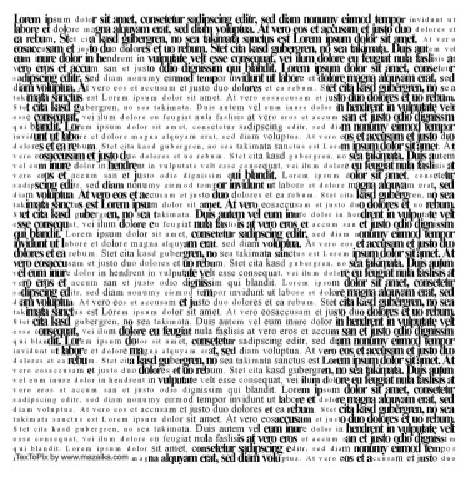
\includegraphics[width=0.5\textwidth]{Bernardi/01x01-eps-converted-to}
%\end{center}
%\caption{This is figure 1 in chapter 1.}
%\end{figure}
%
%\paragraph{Cras adipiscing} sagittis nunc vel luctus. Suspendisse volutpat augue quis erat semper consequat dignissim tellus euismod. Morbi hendrerit, tellus id aliquam iaculis, nibh leo tincidunt eros, vitae varius ligula felis in mi.
%
%\begin{table}
%\caption{Greek Letters.}
%\begin{center}
%\begin{tabular}{llllllll}
%\hline
%$\alpha $  & $ \beta $  & $ \gamma $  & $ \delta $  & $ \epsilon $  & $ \varepsilon $  & $ \zeta $  & $ \eta $ \\
% $ \theta $  &  $ \vartheta $  &  $ \gamma $  &  $ \kappa $  &  $ \lambda $  &  $ \mu $  &  $ \nu $  &  $ \xi $ \\
% $ o $  &  $ \pi $  &  $ \varpi $  &  $ \rho $  &  $ \varrho $  &  $ \sigma $  &  $ \varsigma $  &  $$ \\
% $ \tau $  &  $ \upsilon $  &  $ \phi$ &  $ \varphi $  &  $ \chi $  &  $ \psi $  &  $ \omega$  &  $ $ \\
% &  &  &  &  &  &  & \\
%$ \Gamma $  & $ \Delta $  & $ \Theta $  &  $ \Lambda $  &  $ \Xi $  &  $ \Pi $  &  $ \Sigma $  & $ \Upsilon $ \\
% $ \Phi$ &  $ \Psi $  &  $ \Omega $  &  &  &  &  &\\
%\hline
%\end{tabular}
%\end{center}\end{table}
%
%\begin{figure}[]
%\begin{center}
%
\includegraphics[width=0.6\textwidth]{Bernardi/01x02}
%\end{center}
%\caption{This is figure 2 in chapter 1.}
%\end{figure}
%
%
\bibliographystyle{plain}
\bibliography{Bernardi/References}


